\subsection{Stetigkeit und der Zwischenwertsatz}
Anschaulich wird die Stetigkeit einer Funktion $f:\mathbb{R} \longrightarrow \mathbb{R}$ oft dadurch beschrieben, dass man ihren Graphen zeichnen kann, ohne dabei den Stift abzusetzen. Einmal abgesehen davon, dass man zum mathematisch präzisen Zeichnen eines Graphen einen unendlich dünnen Stift benötigen würde, birgt diese sehr plastische Beschreibung des grundsätzlichen Wesenszugs der Stetigkeit die Gefahr, dass man Funktionen, wie beispielsweise der Tangensfunktion oder auch rationalen Funktionen, die Definitionslücken in $\mathbb{R}$ besitzen, fälschlicherweise ihre Stetigkeit abspricht.


\begin{definition}{Stetigkeit}{Stetigkeit}
    Eine Funktion $f:D\subset \mathbb{R} \longrightarrow \mathbb{R}$ heisst \textbf{stetig an der Stelle $x_0\in D$} genau dann wenn:\newline
    Für alle   $\varepsilon > 0$  existiert ein $\delta_\varepsilon >0$, so dass $$x\in |x-x_0|<\delta_\varepsilon \;\;\; \Longrightarrow \;\;\; |f(x)-f(x_0)|<\varepsilon$$

Die Funktion $f$ heisst \textbf{stetig}, falls sie an jeder Stelle $x_0\in D$ ihres Definitionsbereiches stetig ist.
\end{definition}

\begin{bsp}{Stetigkeit der Quadratfunktion}{}
    Wir wollen zeigen, dass die Funktion $f(x)=x^2$ an der Stelle $x_0=1$ stetig ist.
    \vspace{10cm}
\end{bsp}
\clearpage



Potenzfunktionen mit nicht-negativen Exponenten sind stetig auf ganz $\mathbb{R}$. Da desweiteren Linearkombinationen stetiger Funktionen auch wieder stetig sind, folgt unmittelbar die Stetigkeit aller Polynomfunktionen auf ganz $\mathbb{R}$.

\begin{center}
    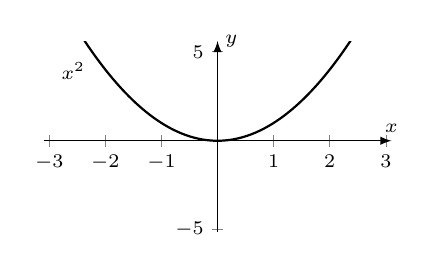
\begin{tikzpicture}
		\scriptsize
		\begin{axis}[			
			width=6cm,
			height=4cm,
			grid=none,
			axis x line=middle,
			axis y line=middle,
			axis line style={-latex},
			x label style={at={(ticklabel* cs:1)},anchor=south},
			y label style={at={(ticklabel* cs:1)},anchor=west},
			xlabel={$x$},
			ylabel={$y$}, 
			xmin=-3.1, xmax=3.1,
			ymin=-5.1, ymax=5.6,
			xtick={-3,-2,...,3},
			ytick={-5,5},
			]
			\addplot [domain=-2.5:2.5, samples=100,thick, black] {x^2} node[pos=0.1, below left] {$x^2$} ;
		\end{axis}
	\end{tikzpicture}
\end{center}

Aber auch die rationalen Funktionen, sind als Quotienten (stetiger) Polynomfunktionen, auf ihrem ganzen Definitionsbereich wieder stetig. Nichtsdestotrotz können aber an den Definitionslücken (also den Nullstellen des Nennerpolynoms) Sprünge im Graphen auftreten.

Ebenso handelt es sich neben der Sinus- und der Kosinusfunktion auch bei der Tangensfunktion um eine auf ihrer gesamten Definitionsmenge stetige Funktion.

Und auch sowohl die Exponentialfunktionen als auch ihre Umkehrfunktionen (die Logarithmusfunktionen) sind auf ihren Definitionsmengen überall stetig.

Die so genannte Gau\ss-Funktion (Abrundungsfunktion) $\left\lfloor x \right\rfloor= \max \{z\in\mathbb{Z}  \, | \, z\le x\}$ ist unstetig in allen $x\in \mathbb{Z}$.

